\documentclass[11pt]{article}

\usepackage[margin=0.84in]{geometry}
\usepackage{amsmath}
\usepackage{amssymb}
\usepackage{booktabs}
\usepackage{graphicx}
\usepackage{microtype}
\usepackage{array}
\usepackage{url}
\usepackage{xcolor}
\usepackage[hidelinks]{hyperref}

\definecolor{passgreen}{HTML}{047857}
\definecolor{failred}{HTML}{B91C1C}
\definecolor{resultblue}{HTML}{1D4ED8}
\newcommand{\pass}{\textcolor{passgreen}{\textbf{PASS}}}
\newcommand{\fail}{\textcolor{failred}{\textbf{FAIL}}}
\newcommand{\code}[1]{\texttt{#1}}

\title{\textbf{Cross-Model Replication of Deterministic ``Neurons''}\\
\large A Frozen Three-Seed TinyLlama Study with an Exact
Parameter-Matched Adapter Control}
\author{Josiah Wilson\\Independent Researcher}
\date{July 27, 2026}

\begin{document}
\maketitle

\begin{abstract}
We test whether a deterministic calculator occupying existing transformer MLP
coordinates transfers from Qwen2.5-0.5B to an independently pretrained
Llama-family model. Every TinyLlama-1.1B parameter was frozen. At decoder layer
15, 28 of 5,632 existing SwiGLU coordinates were assigned a typed interface:
16 learned route, role, and digit channels fed a frozen zero-parameter decimal
adder, and 12 deterministic result channels returned through learned residual
columns. The interface contained 57,344 learned weights
($0.005213\%$ of the 1.10-billion-parameter base). A conventional rank-14
residual adapter at the same layer contained exactly the same number of
learned weights.

The confirmatory protocol froze three seeds, 60 exact-string-disjoint
addition prompts, 60 balanced adversarial negatives, training budgets,
thresholds, and gates before model evaluation. Each implant answered 53/60
additions exactly (88.33\%), versus 0/60 strict exact responses for untouched
TinyLlama and 16/60, 8/60, and 12/60 for the matched adapters. Every seed
recovered exact operands on 54/60. All 53 examples per seed with an active
route and exact operands produced exact calculator digit-plus-end trajectories
and exact final answers. Result-channel ablation reduced every seed to 0/60,
yielding 53 paired causal losses. The three implants nevertheless falsely
routed 12/60, 12/60, and 9/60 adversarial negatives, changing those responses.

The frozen compound protocol failed its accuracy, operand, and
routing/preservation gates. Positive failures and most false routes were
identical across seeds and clustered in unseen semantic families. Phase 8 is
therefore a partial cross-model replication: exact deterministic execution and
native downstream use transferred, but the learned natural-language interface
did not generalize robustly. This negative result makes semantic routing and
operand typing---not the calculator---the immediate bottleneck for the broader
semi-deterministic-AI program.
\end{abstract}

\section*{Technical summary}

\begin{center}
\small
\begin{tabular}{p{0.51\linewidth}rrr}
\toprule
Confirmatory metric & Seed 14,201 & Seed 14,202 & Seed 14,203\\
\midrule
Exact additions & 53/60 & 53/60 & 53/60\\
Direct additions & 26/30 & 26/30 & 26/30\\
Word problems & 27/30 & 27/30 & 27/30\\
Exact operands & 54/60 & 54/60 & 54/60\\
Exact conditional on active route and exact operands
  & 53/53 & 53/53 & 53/53\\
Exact after result ablation & 0/60 & 0/60 & 0/60\\
Paired causal losses & 53/60 & 53/60 & 53/60\\
False routes on adversarial negatives & 12/60 & 12/60 & 9/60\\
Token-exact negative preservation & 48/60 & 48/60 & 51/60\\
Matched-adapter exact additions & 16/60 & 8/60 & 12/60\\
\bottomrule
\end{tabular}
\end{center}

\noindent\textbf{Frozen verdict:} \fail. Three of six technical gates passed;
the procedural no-retraining gate also passed.

\medskip
\noindent\textbf{Mechanistic verdict:} Conditional support. Every correctly
typed calculator execution was exact and decoded exactly, and ablating only
the result coordinates removed every correct implant answer.

\medskip
\noindent\textbf{Generalization verdict:} Failure. The neural interface missed
seven additions per seed and activated on 15--20\% of adversarial negatives.

\section{Motivation and scope}

Flexible neural sequence models and exact algorithms have complementary
strengths. Neural arithmetic architectures and algorithmic-reasoning systems
ask whether explicit structure can improve systematic computation
\cite{trask2018,lindner2023,bounsi2024}. Dietz and Klakow's Integrated Gated
Calculator established direct prior art for a learned calculator module inside
a frozen Llama model \cite{dietz2025}; the present work does not claim the
broad integrated-calculator idea as novel.

The narrower hypothesis proposed by Josiah Wilson is that deterministic
programs can occupy neuron-shaped activation slots inside an otherwise ordinary
network. Surrounding neural computation would learn when and how to encode
state into those slots and how to use their exact outputs. Phase 7 tested this
inside 28 existing coordinates of Qwen2.5-0.5B. It found strong causal evidence
but retained runtime-managed state and several learned-interface failures.

Phase 8 asks one question: does the same single-addition mechanism transfer to
a separately pretrained Llama-family decoder under a frozen, exactly
parameter-matched comparison? It does \emph{not} test arbitrary recurrent
calls, spontaneous discovery during pretraining, multiple operations,
residual-native persistent state, or broad mathematical reasoning.

The longer program is framed as \emph{semi-deterministic AI}: neural
interpretation and flexible learned representations combined with compact,
auditable deterministic mechanisms embedded in native activation pathways.
This report is a controlled arithmetic replication, not evidence that the
broader program is complete.

\section{Model and architecture}

\subsection{Frozen TinyLlama}

Experiments used
\code{TinyLlama/TinyLlama-1.1B-Chat-v1.0} \cite{tinyllama2024}, revision
\begin{sloppypar}
\code{fe8a4ea1ffedaf415f4da2f062534de366a451e6}.
\end{sloppypar}
TinyLlama follows the Llama 2 architecture and tokenizer. The loaded model had
1,100,048,384 parameters, 22 decoder layers, hidden width 2,048, and SwiGLU MLP
width 5,632. All pretrained parameters remained frozen and generation was
greedy.

TinyLlama's SentencePiece tokenizer inserts a word-boundary token when a bare
digit is encoded, although context-independent single-digit vocabulary entries
are used inside natural-language numbers. The shared decimal-token resolver was
generalized to use those exact digit entries. This is tokenizer compatibility,
not a runtime parser: prompt interpretation and operand selection remained
learned from TinyLlama's layer activations.

\subsection{In-place deterministic subspace}

At decoder MLP layer 15, the original SwiGLU computation is
\[
 y_{\mathrm{MLP}}
 = W_{\mathrm{down}}\left(
   \operatorname{SiLU}(W_{\mathrm{gate}}h)
   \odot W_{\mathrm{up}}h\right).
\]
A development census selected 28 low-impact intermediate coordinates. Their
original contribution is separated, leaving all 5,604 unselected coordinates
unchanged. The assigned activation ABI is:

\begin{center}
\small
\begin{tabular}{lrr}
\toprule
Group & Coordinates & Learned weights\\
\midrule
Route: off/add & 2 & $2\times2{,}048=4{,}096$\\
Token role: none/A/B & 3 & $3\times2{,}048=6{,}144$\\
Digit: 0--9/non-digit & 11 & $11\times2{,}048=22{,}528$\\
Result: 0--9/end/pad & 12 & $12\times2{,}048=24{,}576$\\
\midrule
Total & 28 & 57,344\\
\bottomrule
\end{tabular}
\end{center}

The first 16 rows linearly classify route, operand role, and digit from native
layer-15 states. A digit confidence threshold of 0.90 and role/digit agreement
form a typed handshake. Valid operands enter a frozen decimal ripple-carry
adder with zero learned parameters. One-hot result symbols pass through 12
learned residual columns, then through TinyLlama's unchanged downstream
decoder blocks, final normalization, and language head.

When the route is off, the selected coordinates' original MLP contribution is
restored exactly. The route is latched on the first response step; the first
valid operands enter a response-local deterministic register; and a
deterministic counter selects successive result digits. These tensors are
runtime microcircuit state, not learned parameters or residual-native recurrent
state.

\subsection{Parameter-matched learned control}

The ordinary learned control replaces the same layer's MLP output with
\[
  y = y_{\mathrm{base}} +
  W_{\mathrm{up}}^{(a)}
  \operatorname{GELU}(W_{\mathrm{down}}^{(a)}h).
\]
Its bottleneck rank is 14, with no biases:
\[
  2\times2{,}048\times14 = 57{,}344
\]
weights. The up projection is initialized to zero, so the adapter initially
equals the base model exactly. This is a strict learned-parameter match, not a
claim that one adapter design exhausts all possible neural controls.

\section{Protocol}

\subsection{Development and freeze}

Layers 12, 15, and 18 were probed using development-only data. Layer 15
achieved perfect operand-role and digit accuracy, 96.98\% route recall, and
0.83\% route false positives on the probe. Removing its 28 selected coordinates
preserved all 96 development next-token argmaxes; mean KL divergence was
0.000171.

Development pilot seed 14,199 initially reached 35/40 exact additions, 0/40
ablation accuracy, 0/40 false routes, and 40/40 negative preservation.
Retraining only two route rows increased it to 39/40 while retaining 0/40 false
routes. The matched-adapter pilot reached 10/40 additions and 7/40 exact
negative preservation after the subsequently frozen budget. All pilots and
failures were retained.

The implementation was frozen at commit
\code{54dfc1c7086a8fd7595bc5fbd5f52a69d43cb45a}; the protocol was frozen at
\code{495c2f8f28a0df2c60917f47b764b94cc1c90a02} before confirmatory model
training or evaluation.

\subsection{Data}

Training used 1,200 additions and 1,200 adversarial negatives; development used
240 of each. Confirmatory prompts and numeric operand pairs were disjoint from
both. The final set contained:

\begin{itemize}
\item 30 direct addition requests;
\item 30 natural-language addition word problems;
\item 60 adversarial negatives, balanced at 12 each across quoted arithmetic,
      negated requests, multiplication near-misses, factual questions
      containing numbers, and instructions to ignore an embedded sum.
\end{itemize}

All operands had one to four decimal digits. The three conditions received
identical prompts in identical order. Deterministic data tests instantiated
rows before the freeze only to verify counts, category balance, determinism,
and split disjointness; no model was evaluated or tuned on them.

\subsection{Training}

Independent seeds were 14,201, 14,202, and 14,203.

Each implant trained the 16 input rows for 3,000 AdamW updates (batch 256,
learning rate 0.001), the 12 result columns for 200 teacher-forced updates
(batch 1, learning rate 0.01), and then only the two route rows for 3,000
updates (batch 256, learning rate 0.001). The route threshold maximized
development recall subject to a 2.5\% false-positive cap. Result strength was
16.0.

Each matched adapter received 800 AdamW updates (batch 4, learning rate
0.002). Positive examples used teacher-forced exact digits and end token.
Negative examples targeted untouched base's first greedy token. There was no
scheduler and no post-confirmatory retraining.

\subsection{Outcomes and gates}

The primary response budget was eight greedy tokens. Exact numeral-only
addition accuracy, routing, exact first-step operands, exact calculator
trajectory, conditional output, result ablation, adversarial false routes,
token-exact base preservation, latency, sampled memory, and learned parameters
were recorded. Untouched base also received a separate 64-token sensitivity
budget.

Frozen technical gates required:

\begin{enumerate}
\item every seed at least 57/60 exact and mean at least 58/60;
\item every seed at least 57/60 exact operands;
\item every seed at least 50 paired causal losses;
\item every seed at most 2/60 false routes and at least 58/60 exact
      preservation;
\item exact trajectories for all active exact operands and at least 59/60
      conditional decode reliability;
\item every implant seed to exceed both base and its matched adapter.
\end{enumerate}

A seventh procedural gate prohibited unreported replacement, prompt revision,
threshold change, or post-confirmatory retraining.

\section{Results}

\subsection{Accuracy and controls}

\begin{figure}[t]
\centering
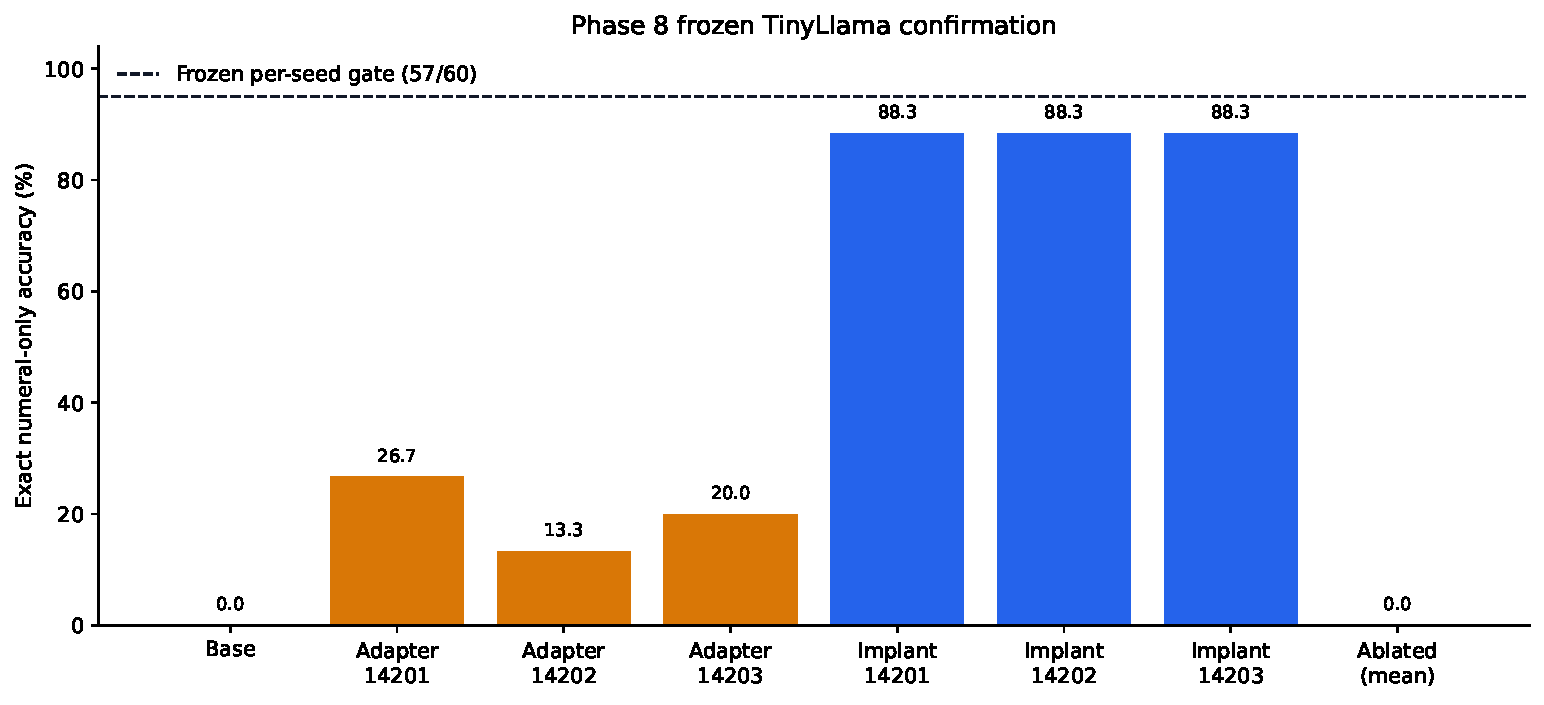
\includegraphics[width=\linewidth]{../phase8_figures/condition_accuracy.pdf}
\caption{Strict exact numeral-only accuracy. The dashed line is the frozen
per-seed implant gate. Untouched base and result ablation are zero.}
\label{fig:accuracy}
\end{figure}

Every implant seed achieved 53/60 exact additions (88.33\%); exact prompt
decisions were identical across seeds. Untouched base produced 0/60 strict
exact responses under the same budget. With 64 tokens, it still produced 0/60
strict responses but recovered the correct final integer in 3/60 outputs.

Matched adapters achieved 16/60 (26.67\%), 8/60 (13.33\%), and 12/60
(20.00\%). Implant gains over the seed-matched adapters were 61.67, 75.00, and
68.33 percentage points. A secondary prompt-clustered bootstrap gave an
implant accuracy interval of [80.0\%, 95.0\%] and implant-minus-adapter
interval of [57.22, 78.89] percentage points. These are descriptive intervals:
prompts are not independent model replications, and the implant seeds made
identical exactness decisions.

\subsection{Causal deterministic execution}

Each implant recovered exact operands on 54/60 prompts. Fifty-three examples
per seed had both an active route and exact registered operands. Every one
produced the exact deterministic digit-plus-end trajectory and exact final
answer. No conditional downstream decoding error occurred.

Zeroing only the 12 calculator-result coordinates reduced every seed from
53/60 exact to 0/60. Thus all 53 correct answers per seed were paired causal
losses. This result is stronger than observing that the embedded Python
calculation returned correct sums: the learned neural state had to frame the
operands, the fixed activation subspace had to produce result symbols, and
TinyLlama's frozen downstream network had to decode them.

\subsection{Positive failure taxonomy}

\begin{figure}[t]
\centering
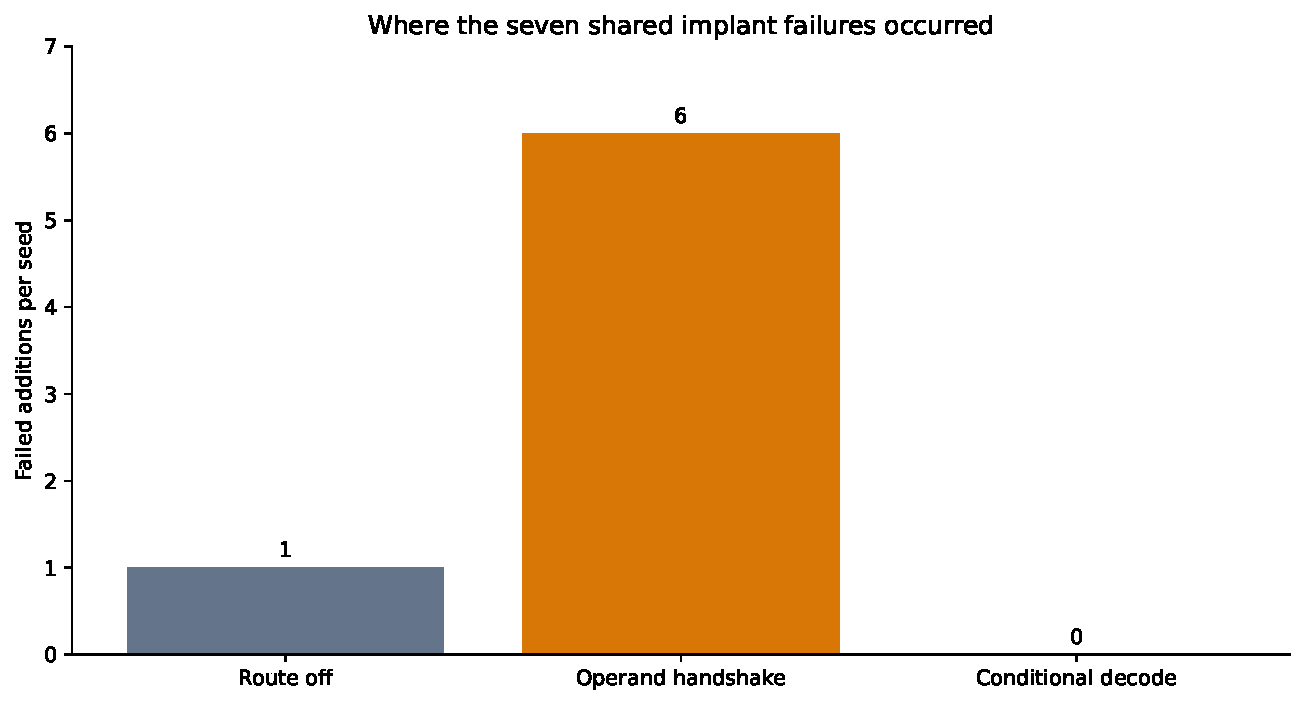
\includegraphics[width=0.88\linewidth]{../phase8_figures/positive_failure_taxonomy.pdf}
\caption{All three seeds shared the same seven failed additions. No failure
occurred after a valid deterministic trajectory.}
\label{fig:positivefailures}
\end{figure}

The same seven prompts failed in every seed:

\begin{itemize}
\item one direct prompt predicted route off;
\item three reversed-order ``move forward'' prompts predicted addition but
      failed the typed operand handshake;
\item three prompts from one unseen telescope word-problem family failed
      operand recovery; two activated with wrong registered digits and
      consequently emitted wrong sums;
\item zero failures occurred after an active route with exact operands.
\end{itemize}

This decomposition localizes the positive shortfall to the learned interface,
not to ripple-carry execution or downstream use of correct result symbols.

\subsection{Adversarial routing and preservation}

\begin{figure}[t]
\centering
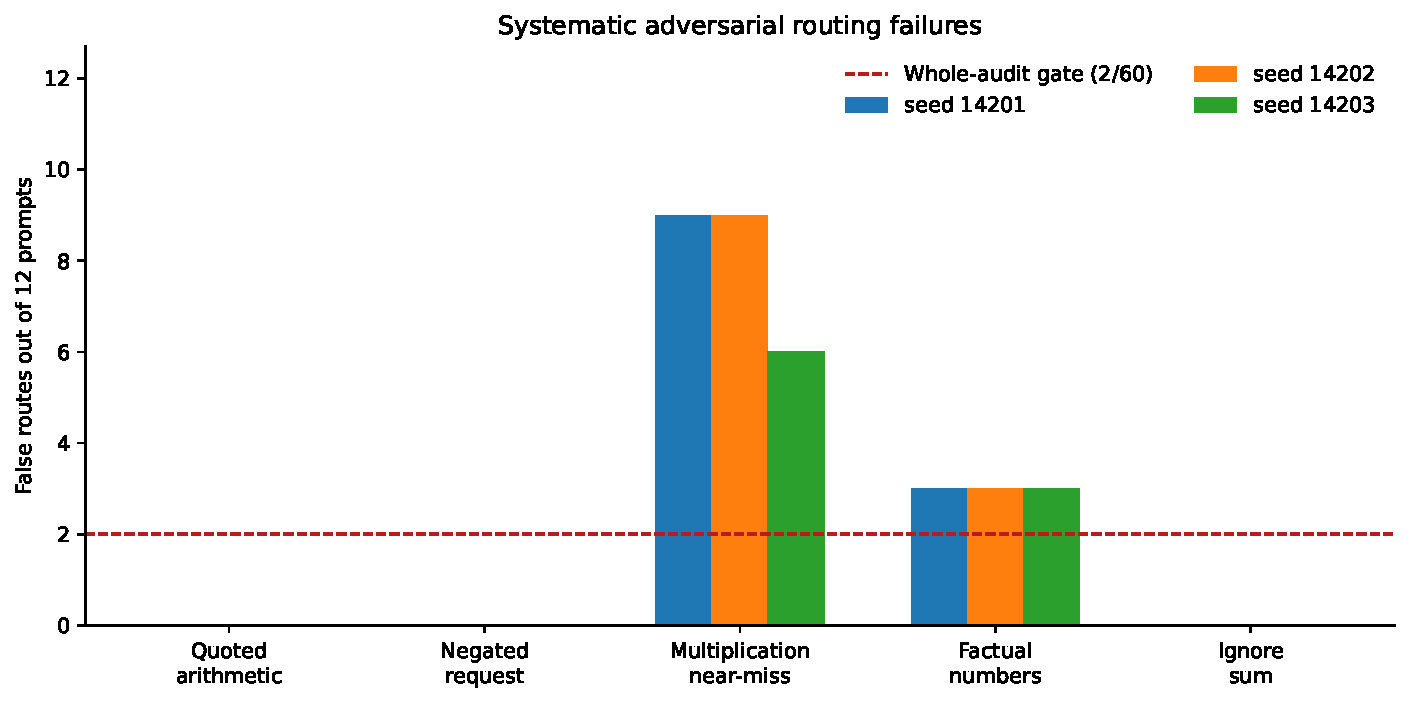
\includegraphics[width=\linewidth]{../phase8_figures/negative_false_routes.pdf}
\caption{False routes by balanced adversarial category. The horizontal line is
the whole-audit maximum, shown for reference; it is not a per-category gate.}
\label{fig:negatives}
\end{figure}

Seeds 14,201 and 14,202 falsely routed 12/60 negatives; seed 14,203 falsely
routed 9/60. Exact preservation was 48/60, 48/60, and 51/60 because route-off
examples restored the base path exactly.

Quoted arithmetic, negated requests, and explicit ignore-sum instructions had
zero false routes in every seed. Multiplication near-misses caused 9/12, 9/12,
and 6/12 false routes; one factual-number family caused another 3/12 in every
seed. False multiplication routes generally emitted the operands' \emph{sum},
directly demonstrating incorrect semantic activation of the deterministic
addition circuit.

\subsection{Efficiency}

The implant and matched adapter each learned 57,344 weights, or 0.005213\% of
the base parameter count. The deterministic calculator learned none.

Median generation latency was 0.712 seconds for untouched base, 0.417--0.476
seconds for matched adapters, and 0.714--0.786 seconds for implants on the
recorded Apple M4 implementation. Adapter timing is confounded by incorrect
early terminations; all conditions also used deliberately uncached
prefix-recomputation. The maximum sampled allocated MPS memory was 4.40 GB.
This is a post-generation sample maximum, not a device-driver peak watermark.

\section{Frozen gate audit}

\begin{center}
\small
\begin{tabular}{p{0.56\linewidth}cc}
\toprule
Gate & Outcome & Evidence\\
\midrule
Exact accuracy & \fail & 53/60 each; required 57/60\\
Exact operands & \fail & 54/60 each; required 57/60\\
Paired causal ablation & \pass & 53/60 each; required 50/60\\
Routing and preservation & \fail & 9--12 false routes; allowed 2\\
Conditional trajectory and decode & \pass & 53/53 each\\
Beats base and matched adapter & \pass & true in every seed\\
No outcome-responsive changes & \pass & no replacement or retraining\\
\bottomrule
\end{tabular}
\end{center}

The compound protocol failed. Reporting the causal and comparative successes
does not convert the frozen verdict into a pass.

\section{Discussion}

\subsection{What transferred}

The narrow deterministic mechanism transferred across two distinct pretrained
model families. TinyLlama's native states could supply typed operands to 28
repurposed MLP coordinates, a zero-parameter calculator could write exact
symbols into the same activation pathway, and unchanged downstream layers
could convert those symbols to text. Exact ablation and exact conditional
decoding provide causal evidence that the correct answers used the implant.

The matched comparison also matters. With precisely the same learned weight
budget, an ordinary nonlinear residual adapter was far less accurate. This
supports the efficiency hypothesis in this particular training design:
offloading the transition itself to a fixed algorithm leaves learned weights
to solve interpretation and representation.

\subsection{What did not transfer}

The semantic interface did not survive the frozen distribution shift.
Three independently initialized seeds converged to the same seven positive
errors and nearly the same negative errors. That agreement is not evidence of
robust replication; it indicates systematic blind spots imposed by training
families and a linear route/role/digit interface.

Operation contrast was especially weak. The router often treated unfamiliar
multiplication wording as an addition request even when ``product'' or
``multiplication'' was explicit. Operand typing also overfit familiar semantic
order and word-problem language. The deterministic component faithfully
executed the wrong requested transition when the neural interface supplied the
wrong type.

\subsection{Limitations}

\begin{itemize}
\item The interface received explicit route, role, digit, and output
      supervision; spontaneous discovery from language-model loss is untested.
\item Runtime state is managed by a route latch, operand register, and result
      counter outside persistent residual activations.
\item Only nonnegative one-to-four-digit addition and one call per response
      were tested.
\item The matched adapter is one fair parameter-count control, not the
      strongest possible learned architecture or hyperparameter search.
\item Base strict exactness is sensitive to instruction following; the
      64-token final-integer sensitivity partly addresses verbosity but not
      every alternative scoring rule.
\item The study uses one TinyLlama revision, one selected layer, one hardware
      environment, and only three interface seeds.
\item Latency uses no KV cache and sampled MPS memory is not a true device
      peak.
\end{itemize}

\subsection{Next experiment}

The next phase should improve the neural interface before adding operations.
Development training should include hard operation contrasts, especially
novel multiplication phrasing and quantitative factual questions, plus
semantic-role diversity for reversed-order and unfamiliar word-problem
templates. A new exact-string-disjoint audit must be frozen before evaluating
that repair. The current failed confirmation remains immutable.

Only after a clean interface replication should the program move to
residual-native persistent state, repeated invocation during reasoning, and
broader deterministic mechanisms. Board-game transitions are no longer the
designated next domain; the program now prioritizes the foundations of
semi-deterministic AI across useful scientific and engineering processes.

\section{Reproducibility}

The frozen protocol is
\path{PHASE8_SECOND_MODEL_REPLICATION_PROTOCOL.md}. Raw prompt-level outputs,
token traces, and condition metrics are retained in
\path{phase8_results/confirmation.json}; the flat table is
\path{phase8_results/confirmation_rows.csv}; post-hoc decomposition is
\path{phase8_results/analysis.json}.

SHA-256 values:

\begin{sloppypar}
\begin{itemize}
\scriptsize
\item confirmation JSON:
\code{203c72f40d42b7a0901e1ce663bbd29b232963ffc49de4822b3ab14f8af39877};
\item confirmation CSV:
\code{f38bde1b055935be1eac1d4ce3fa0dadcf542bb30570af2bef610967b280361e};
\item post-hoc analysis:
\code{6c1ec90acc25d974ca042c92259e20e2cc62149895faf003c96d4a5ff9b8dd07};
\item implant training record:
\code{6fc7f81c074a3acdc8a5945ac63683807e7e34a7b0ba38c6dcc0d9a1544c72d2};
\item matched-adapter training record:
\code{fde0f392f0ebde4ce6f51b1e526d3a93f732a6234894e3f2199ba950014b444b}.
\end{itemize}
\end{sloppypar}

Checkpoint tensor-shape verification found 32,768 learned input weights and
24,576 learned result weights in every implant. A staged-training metadata
field reports only 24,576 because it counted tensors whose
\code{requires\_grad} flag remained true after the output stage; the raw
checkpoints and analysis record the correct architectural total of 57,344.

Experiments ran on macOS 26.5.2 arm64 with Python 3.12.12, PyTorch 2.13.0,
Transformers 4.57.6, and Apple MPS. Large checkpoints remain in ignored local
artifact directories; their hashes are retained in tracked training and
evaluation records.

\section{Conclusion}

Phase 8 did not pass its frozen replication protocol. It did show that a
deterministic neuron-shaped arithmetic subspace can be installed in a
Llama-family model, can be driven by learned native activations, can be decoded
by frozen downstream layers, and can outperform an exactly parameter-matched
learned residual. All correct answers were causally dependent on the result
coordinates.

The result also exposes the central obstacle. A perfect calculator does not
make a semi-deterministic model reliable when learned intent routing and state
typing are brittle. The proper scientific conclusion is therefore partial
cross-model support and failed robust generalization. That negative result
sets a clearer next target than adding more deterministic machinery: make the
neural interface understand when and what to compute.

\section*{Acknowledgment}

The deterministic-neuron hypothesis and semi-deterministic-AI research
direction were proposed by Josiah Wilson. Experimental design, implementation,
local execution, analysis, and drafting were conducted collaboratively with
OpenAI Codex under his direction. All failed gates and observed errors
described here are retained.

\begin{thebibliography}{5}

\bibitem{trask2018}
A. Trask, F. Hill, S. Reed, J. Rae, C. Dyer, and P. Blunsom.
\newblock Neural Arithmetic Logic Units.
\newblock \emph{NeurIPS}, 2018.
\newblock \url{https://arxiv.org/abs/1808.00508}.

\bibitem{lindner2023}
D. Lindner, J. Kram\'{a}r, S. Farquhar, M. Rahtz, T. McGrath, and V. Mikulik.
\newblock Tracr: Compiled Transformers as a Laboratory for Interpretability.
\newblock \emph{NeurIPS}, 2023.
\newblock \url{https://arxiv.org/abs/2301.05062}.

\bibitem{bounsi2024}
W. Bounsi, B. Ibarz, A. Dudzik, J. Hamrick, L. Markeeva, A. Vitvitskyi,
R. Pascanu, and P. Veli\v{c}kovi\'{c}.
\newblock Transformers Meet Neural Algorithmic Reasoners.
\newblock 2024.
\newblock \url{https://arxiv.org/abs/2406.09308}.

\bibitem{tinyllama2024}
P. Zhang, G. Zeng, T. Wang, and W. Lu.
\newblock TinyLlama: An Open-Source Small Language Model.
\newblock 2024.
\newblock \url{https://arxiv.org/abs/2401.02385}.

\bibitem{dietz2025}
F. Dietz and D. Klakow.
\newblock IGC: Integrating a Gated Calculator into an LLM to Solve Arithmetic
Tasks Reliably and Efficiently.
\newblock 2025.
\newblock \url{https://arxiv.org/abs/2501.00684}.

\end{thebibliography}

\end{document}
